% Options for packages loaded elsewhere
\PassOptionsToPackage{unicode}{hyperref}
\PassOptionsToPackage{hyphens}{url}
%
\documentclass[
]{memoir}
\usepackage{lmodern}
\usepackage{amssymb,amsmath}
\usepackage{ifxetex,ifluatex}
\ifnum 0\ifxetex 1\fi\ifluatex 1\fi=0 % if pdftex
  \usepackage[T1]{fontenc}
  \usepackage[utf8]{inputenc}
  \usepackage{textcomp} % provide euro and other symbols
\else % if luatex or xetex
  \usepackage{unicode-math}
  \defaultfontfeatures{Scale=MatchLowercase}
  \defaultfontfeatures[\rmfamily]{Ligatures=TeX,Scale=1}
\fi
% Use upquote if available, for straight quotes in verbatim environments
\IfFileExists{upquote.sty}{\usepackage{upquote}}{}
\IfFileExists{microtype.sty}{% use microtype if available
  \usepackage[]{microtype}
  \UseMicrotypeSet[protrusion]{basicmath} % disable protrusion for tt fonts
}{}
\makeatletter
\@ifundefined{KOMAClassName}{% if non-KOMA class
  \IfFileExists{parskip.sty}{%
    \usepackage{parskip}
  }{% else
    \setlength{\parindent}{0pt}
    \setlength{\parskip}{6pt plus 2pt minus 1pt}}
}{% if KOMA class
  \KOMAoptions{parskip=half}}
\makeatother
\usepackage{xcolor}
\IfFileExists{xurl.sty}{\usepackage{xurl}}{} % add URL line breaks if available
\IfFileExists{bookmark.sty}{\usepackage{bookmark}}{\usepackage{hyperref}}
\hypersetup{
  pdftitle={Prácticas de Ingeniería de Servidores},
  pdfauthor={Alonso Bueno Herrero},
  hidelinks,
  pdfcreator={LaTeX via pandoc}}
\urlstyle{same} % disable monospaced font for URLs
\usepackage{longtable,booktabs}
% Correct order of tables after \paragraph or \subparagraph
\usepackage{etoolbox}
\makeatletter
\patchcmd\longtable{\par}{\if@noskipsec\mbox{}\fi\par}{}{}
\makeatother
% Allow footnotes in longtable head/foot
\IfFileExists{footnotehyper.sty}{\usepackage{footnotehyper}}{\usepackage{footnote}}
\makesavenoteenv{longtable}
\usepackage{graphicx,grffile}
\makeatletter
\def\maxwidth{\ifdim\Gin@nat@width>\linewidth\linewidth\else\Gin@nat@width\fi}
\def\maxheight{\ifdim\Gin@nat@height>\textheight\textheight\else\Gin@nat@height\fi}
\makeatother
% Scale images if necessary, so that they will not overflow the page
% margins by default, and it is still possible to overwrite the defaults
% using explicit options in \includegraphics[width, height, ...]{}
\setkeys{Gin}{width=\maxwidth,height=\maxheight,keepaspectratio}
% Set default figure placement to htbp
\makeatletter
\def\fps@figure{htbp}
\makeatother
\setlength{\emergencystretch}{3em} % prevent overfull lines
\providecommand{\tightlist}{%
  \setlength{\itemsep}{0pt}\setlength{\parskip}{0pt}}
\setcounter{secnumdepth}{5}
\usepackage{booktabs}
\usepackage[]{natbib}
\bibliographystyle{apalike}

\title{Prácticas de Ingeniería de Servidores}
\author{Alonso Bueno Herrero}
\date{Curso 2019-20. Última modificación: 2021-09-24}

\begin{document}
\maketitle

{
\setcounter{tocdepth}{1}
\tableofcontents
}
\hypertarget{p1}{%
\chapter{\texorpdfstring{Instalación de servidores: \textbf{\emph{Ubuntu Server}} y \textbf{\emph{centOS}}}{Instalación de servidores: Ubuntu Server y centOS}}\label{p1}}

\hypertarget{objetivos-de-la-pruxe1ctica}{%
\section{Objetivos de la práctica}\label{objetivos-de-la-pruxe1ctica}}

Objetivos mínimos:

\begin{enumerate}
\def\labelenumi{\arabic{enumi}.}
\tightlist
\item
  Familiarizarse con distintos Sistemas Operativos (SOs) usados en servidores.
\item
  Conocer alternativas comerciales para tener un servidor.
\item
  Configurar unidades de disco RAID y LVM.
\item
  Configurar una red local de máquinas virtuales.
\end{enumerate}

\hypertarget{sesiuxf3n-1-instalaciuxf3n-de-ubuntu-server-y-centos}{%
\section{Sesión 1: Instalación de Ubuntu Server y centOS}\label{sesiuxf3n-1-instalaciuxf3n-de-ubuntu-server-y-centos}}

\hypertarget{conceptos-buxe1sicos}{%
\subsection{Conceptos básicos}\label{conceptos-buxe1sicos}}

Repasamos los siguientes conceptos básicos que conviene conocer antes de iniciar las tareas de esta sesión:

\begin{enumerate}
\def\labelenumi{\arabic{enumi}.}
\item
  Servidor, como un sistema informático que recibe peticiones y da respuestas a las mismas.
\item
  Tecnología de servidores, distinguiendo:

  \begin{enumerate}
  \def\labelenumii{\alph{enumii}.}
  \tightlist
  \item
    \textbf{\emph{Hosting}} dedicado:es una configuración de alojamiento en el que se dedica un servidor a una sola organización o para un solo propósito, como una página web. No escalable.
  \item
    \textbf{\emph{VPS}} (Virtual Private Server), donde varias MV comparten una serie de recursos hardware (Disco Duro, RAM, CPU, \ldots).
  \item
    \textbf{\emph{Serverless}} (servicios en la nube), las aplicaciones montan ahí sus recursos y todas las tareas de administración de sistema están abstraídas para el usuario hasta el punto que él no tiene que preocuparse de las mismas. Es el modelo más actual por su alta capacidad de escalabilidad.
  \end{enumerate}
\item
  Una tecnología de servidores basada en contenedores se caracteriza porque cada uno de estos contenedores se interpreta como una MV, sólo que cada una de esas MV son aplicaciones sobre el SO anfitrión, en tanto en cuanto:

  \begin{itemize}
  \tightlist
  \item
    Los contenedores están (pueden estar) interconectados entre sí,
  \item
    Puedo añadir nuevos contenedores dinámicamente e ir conectándolos a otros que estén en activo (arrancados, funcionando).
  \end{itemize}

  Un ejemplo es un servidor web donde un contenedor C1 contiene el motor web, otro C2 contiene la base de datos y el C3, que contendría el intérprete de peticiones web.
\item
  La tecnología \emph{RAID} surge como solución a la problemática del precio del almacenamiento. Las siglas se refieren a \textbf{\emph{Redundant Array of Independent Disks}} (Almacén Redundante de Discos Independientes). Existen diversos tipos de tecnologías RAID, las más importantes son RAID-0 y RAID-1:

  \begin{enumerate}
  \def\labelenumii{\alph{enumii}.}
  \tightlist
  \item
    \emph{RAID-0}. Un RAID-0 distribuye los datos equitativamente entre dos o más discos (usualmente se ocupa el mismo espacio en dos o más discos) sin información de paridad que proporcione redundancia. Es importante señalar que el RAID 0 no es redundante. Un RAID 0 puede ser creado con discos de diferentes tamaños, pero el espacio de almacenamiento añadido al conjunto estará limitado por el tamaño del disco más pequeño (por ejemplo, si se hace un conjunto dividido con un disco de 450 GB y otro de 100 GB, el tamaño del conjunto resultante será sólo de 200 GB, ya que cada disco aporta 100 GB).
  \item
    Un RAID 1 crea una copia exacta (o espejo) de un conjunto de datos en dos o más discos. Esto resulta útil cuando queremos tener más seguridad desaprovechando capacidad, ya que si perdemos un disco, tenemos el otro con la misma información. Un conjunto RAID 1 sólo puede ser tan grande como el más pequeño de sus discos. Un RAID 1 clásico consiste en dos discos en espejo, lo que incrementa exponencialmente la fiabilidad respecto a un solo disco; es decir, que para que el conjunto falle es necesario que lo hagan todos sus discos.
  \item
    \textbf{Ejercicio} Busca información sobre los tipos de RAID siguientes: RAID-10, RAID-5 y RAID-6.
  \end{enumerate}
\end{enumerate}

\begin{figure}

{\centering 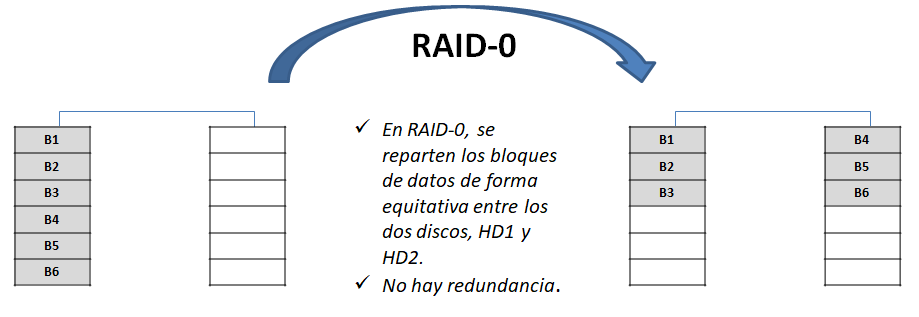
\includegraphics[width=0.9\linewidth]{images/raid0} 

}

\caption{Configuración de RAID-0. Elaboración propia.}\label{fig:rmarkdown}
\end{figure}

\begin{enumerate}
\def\labelenumi{\arabic{enumi}.}
\setcounter{enumi}{4}
\tightlist
\item
  Sistema de archivos

  \begin{enumerate}
  \def\labelenumii{\alph{enumii}.}
  \tightlist
  \item
    Sistema de archivos \emph{ext2}: principales características:

    \begin{itemize}
    \tightlist
    \item
      No admite Journaling
    \item
      Adecuado para tarjetas SD y unidades USB, ya que tiene un alto rendimiento y escritura baja (ya que el registro en diario no está disponible). USB y almacenamiento SD están limitados con ciclos de escritura por lo tanto su mejor ajuste para ellos.
    \item
      Límites: Tamaño de archivo individual de 16 GB a 2 TB.
    \item
      Tamaño del sistema de archivos de 2TB a 32TB.
    \end{itemize}
  \item
    Sistema de archivos ext4

    \begin{itemize}
    \tightlist
    \item
      Soporta Journaling
    \item
      Muchas de las nuevas características introducidas. Extents, Compatibilidad con versiones anteriores, Pre-asignación persistente, Asignación diferida, Número ilimitado de subdirectorios, Suma de comprobación del diario, Comprobación FS más rápida, Encriptación transparente.
    \item
      Límites: Tamaño de archivo individual de 16GB a 16TB. Tamaño del sistema de archivos hasta 1EB.
    \item
      No es necesario actualizar el sistema de archivos. Debido a la compatibilidad hacia atrás, ext2, ext3 se puede montar directamente como ext4.
    \end{itemize}
  \end{enumerate}
\end{enumerate}

\hypertarget{proceso-de-instalaciuxf3n-de-ubuntu-server-16.04}{%
\subsection{Proceso de instalación de Ubuntu Server 16.04}\label{proceso-de-instalaciuxf3n-de-ubuntu-server-16.04}}

\hypertarget{sesiuxf3n-2-ampliaciuxf3n-de-capacidad-para-un-usuario-en-el-servidor-centos.}{%
\section{\texorpdfstring{Sesión 2: Ampliación de capacidad para un usuario en el servidor \textbf{\emph{centOS}}.}{Sesión 2: Ampliación de capacidad para un usuario en el servidor centOS.}}\label{sesiuxf3n-2-ampliaciuxf3n-de-capacidad-para-un-usuario-en-el-servidor-centos.}}

En este caso, la idea es que, una vez instalado el servidor de centOS en el disco por defecto que nos crea VirtualBox, añadamos más capacidad a la ``carpeta'' de ese usuario concreto.

Para estas operaciones habrá que tener en cuenta algunas consideraciones y delicadezas de centOS con respecto a Ubuntu. Pero ya las iremos viendo\ldots{}

\hypertarget{contextualizaciuxf3n-del-escenario-profesional}{%
\subsection{Contextualización del escenario profesional}\label{contextualizaciuxf3n-del-escenario-profesional}}

El escenario profesional es el siguiente: En esta ocasión, en la empresa en la que le acaban de contratar tenían adquirido un servidor y su predecesor había realizado la instalación del S.O. CentOS, según le han comentado los compañeros, él solía hacer instalaciones por defecto y luego aplicar scripts de configuración. Sin más información, nuestro jefe nos informa que esa máquina va a alojar unos cursos con vídeos de alta calidad y relativamente largos. Por tanto, viendo la configuración del sistema, prevemos que /var necesitará más espacio, incluso es conveniente asignarle un LV exclusivamente. Para ello, incluiremos un nuevo disco y configuraremos LVM para que /var se monte en el nuevo VL que crearemos para él.

\hypertarget{pasos-previos-instalaciuxf3n-de-centos}{%
\subsection{\texorpdfstring{Pasos previos: instalación de \textbf{\emph{centOS}}}{Pasos previos: instalación de centOS}}\label{pasos-previos-instalaciuxf3n-de-centos}}

\begin{quote}
Recuerda que al instalar centOS hay que crear el usuario con su clave y darle permisos de administrador. Además tienes que establecer contraseña de root para poder hacer todo lo siguiente.
\end{quote}

\hypertarget{procedimiento}{%
\subsection{Procedimiento}\label{procedimiento}}

Pasos a realizar:

\begin{enumerate}
\def\labelenumi{\arabic{enumi}.}
\tightlist
\item
  Una vez hecha la instalación por defecto, y al iniciar sesión en el servidor, se nos proporciona el siguiente \emph{sistema de particiones} sobre el único disco que tenemos, de 8 GB, que le habíamos proporcionado (ver figura \ref{fig:a}).
\end{enumerate}

\begin{figure}

{\centering 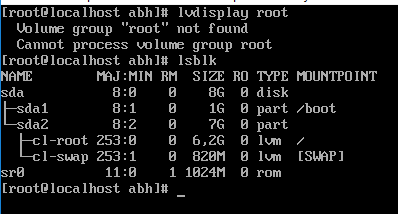
\includegraphics[width=0.6\linewidth]{images/a} 

}

\caption{Situación de particionado del primer disco tras instalar centOS con las opciones por defecto.}\label{fig:a}
\end{figure}

Es decir, que el volumen físico \texttt{sda2}tiene 7GB y en él se ubica el VG llamado \texttt{cl}, donde están los volúmenes lógicos \texttt{root} (de 6,2 GB) y \texttt{swap} (de 820 MB).

\begin{enumerate}
\def\labelenumi{\arabic{enumi}.}
\setcounter{enumi}{1}
\tightlist
\item
  Añadamos el nuevo disco y configurémoslo para que \texttt{/var} tenga ese espacio extra (todo esto tiene detrás un proceso relativamente corto que iremos viendo).
\end{enumerate}

Por ahora, apagamos el ordenador (comando \texttt{poweroff}), añadimos el nuevo disco a nuestra Máquina Virtual y arrancamos. La situación tras añadir el nuevo disco ``físico'' y hacer \texttt{lsblk} es se ve en la figura \ref{fig:b}.

\begin{figure}

{\centering 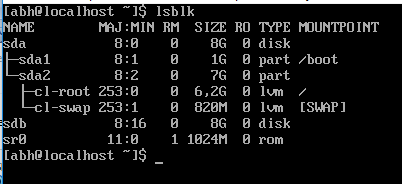
\includegraphics[width=0.6\linewidth]{images/b} 

}

\caption{Situación tras aña}\label{fig:b}
\end{figure}

\begin{enumerate}
\def\labelenumi{\arabic{enumi}.}
\setcounter{enumi}{2}
\tightlist
\item
  Como vemos, aparece el disco \texttt{sdb}, que es el nuevo disco que hemos añadido, pero vemos que no tiene ningún PV (volumen físico) asociado, con lo cual es como si ese espacio lo tuviéramos inútil al completo. Comprobémoslo con la(s) orden(es) de LVM que nos informa(n) de los volúmenes físicos existentes en nuestro sistema: \texttt{pvdisplay} o de forma resumida, \texttt{pvs} (ver figura \ref{fig:c}).
\end{enumerate}

\begin{figure}

{\centering 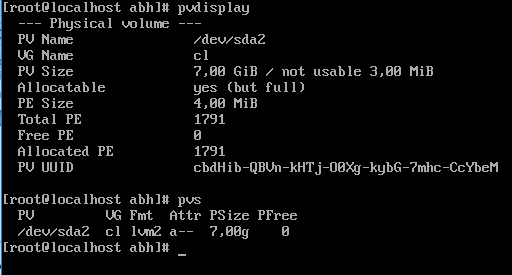
\includegraphics[width=0.6\linewidth]{images/c} 

}

\caption{Mostrando los volúmenes físicos actuales. }\label{fig:c}
\end{figure}

Y vemos que en efecto no refleja nada sobre el segundo disco creado.

\begin{enumerate}
\def\labelenumi{\arabic{enumi}.}
\setcounter{enumi}{3}
\tightlist
\item
  Lo primero que vamos a hacer es definir el volumen físico asociado a ese nuevo disco, para ello usaremos el comando \texttt{pvcreate} (ver figura \ref{fig:d}).
\end{enumerate}

\begin{figure}

{\centering 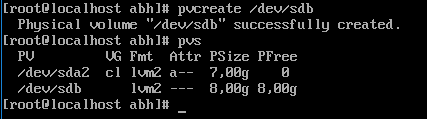
\includegraphics[width=0.7\linewidth]{images/d} 

}

\caption{Creación del nuevo volumen físico `sdb` y comprobación de que se ha creado con la orden `pvs`.}\label{fig:d}
\end{figure}

\begin{enumerate}
\def\labelenumi{\arabic{enumi}.}
\setcounter{enumi}{4}
\tightlist
\item
  Ahora hay que extender el Grupo de Volúmenes (VG) llamado \texttt{cl} con este nuevo volumen físico (recordemos la jerarquía de particiones y nomenclatura que establecía LVM) mediante la orden \texttt{vgextend}, y comprobamos que lo hemos hecho bien en la figura \ref{fig:e}.
\end{enumerate}

\begin{figure}

{\centering 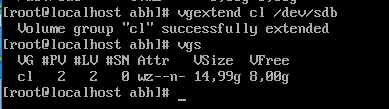
\includegraphics[width=0.7\linewidth]{images/e} 

}

\caption{Extendiendo el grupo de volúmenes `cl` y comprobando que lo hemos hecho bien con el comando `vgs`.}\label{fig:e}
\end{figure}

Y vemos que ya el campo \texttt{\#PV} aparece con el valor \texttt{2}.

\begin{enumerate}
\def\labelenumi{\arabic{enumi}.}
\setcounter{enumi}{5}
\tightlist
\item
  Ahora vamos a \textbf{crear el nuevo volumen lógico} donde almacenar los datos que queremos, y que montaremos en \texttt{/var} (ver figura \ref{fig:f}):
\end{enumerate}

\begin{figure}

{\centering 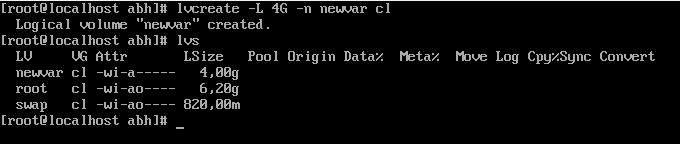
\includegraphics[width=0.9\linewidth]{images/f} 

}

\caption{Creación del volumen lógico con la orden `lvcreate`.}\label{fig:f}
\end{figure}

Y queda comprobado que se ha creado bien.

\begin{enumerate}
\def\labelenumi{\arabic{enumi}.}
\setcounter{enumi}{6}
\tightlist
\item
  Ahora vamos a asignarle un \textbf{sistema de ficheros} mediante el comando \texttt{mkfs} con la opción \texttt{–t} para indicarle el tipo de Sistema de Archivos que le vamos a dar (en este caso, \emph{ext4}), tal y como se muestra en la figura \ref{fig:g}.
\end{enumerate}

\begin{figure}

{\centering 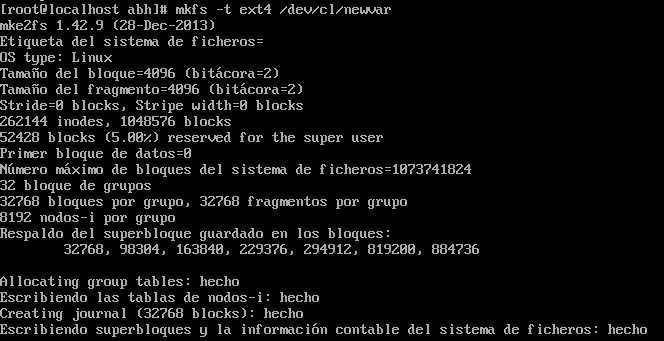
\includegraphics[width=0.8\linewidth]{images/g} 

}

\caption{Asignando un sistema de archivos al nuevo volumen lógico.}\label{fig:g}
\end{figure}

\begin{enumerate}
\def\labelenumi{\arabic{enumi}.}
\setcounter{enumi}{7}
\tightlist
\item
  A continuación, tenemos que \textbf{montar el volumen lógico \texttt{newvar} para que esté accesible}\footnote{Una analogía para recordar por qué montar un volumen: cuando conectamos una unidad de almacenamiento o un lector de DVD, el sistema tiene que crearle lo que se denomina un punto de montaje para poderlo utilizar. Este punto de montaje en casos de discos duros y pendrive's, suele ser una carpeta que creamos manualmente en el sistema o nos lo crea él mismo automáticamente en una partición denominada \texttt{/media} en distribuciones basadas en Ubuntu. En nuestro caso, directamente las montamos sobre \texttt{/mnt/\textless{}dir\_pto\_montaje\textgreater{}}.} sobre un punto de montaje que vamos a crearnos y que se va a llamar \texttt{/mnt/newvar}:
\end{enumerate}

\begin{verbatim}
mkdir /mnt/newvar                           # crear carpeta aux. ` 
mount /dev/cl/newvar /mnt/newvar            # montar VL en aux.
\end{verbatim}

\begin{enumerate}
\def\labelenumi{\arabic{enumi}.}
\setcounter{enumi}{8}
\tightlist
\item
  Vamos a comprobar que el montaje ha sido satisfactorio. Para ello volvemos a ejecutar \texttt{mount} pero sin ninguna opción (o bien con \texttt{\$\ mount\ \textbar{}\ grep\ var}, para que marque en color donde está \texttt{/var}), y en la última línea debería aparecer nuestro dispositivo newvar montado sobre \texttt{/mnt/newvar}, tal y como se muestra en la figura \ref{fig:h}.
\end{enumerate}

\begin{figure}

{\centering 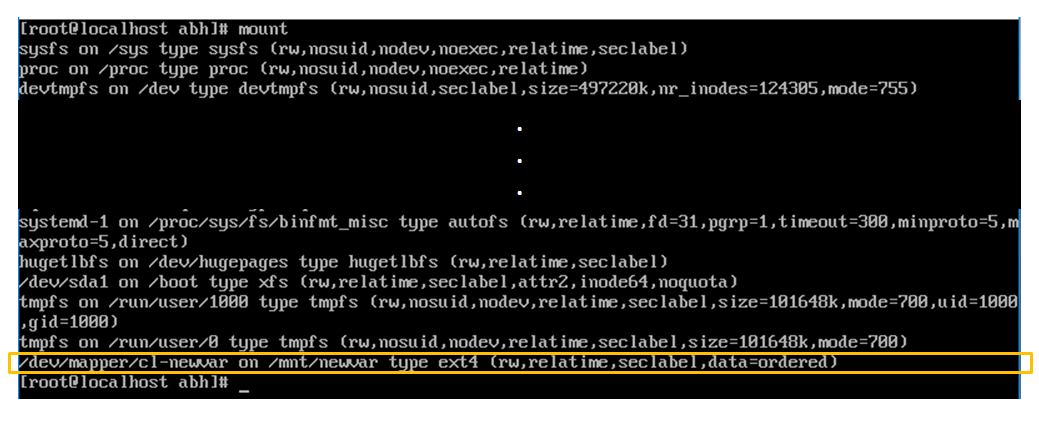
\includegraphics[width=0.8\linewidth]{images/h} 

}

\caption{Fragmento (inicio y fin) de la orden `mount` tras montar newvar sobre el directorio auxiliar `/mnt/newvar` recién creado.}\label{fig:h}
\end{figure}

\begin{enumerate}
\def\labelenumi{\arabic{enumi}.}
\setcounter{enumi}{9}
\tightlist
\item
  Ahora habría que copiar el contenido de /var, que es lo que queremos ampliar, en \texttt{/mnt/newvar}. Pero para evitar que otros usuarios hagan operaciones \emph{r/w} mientras se hace esto, vamos a hacerlo de manera atómica, usando el modo \textbf{AISLADO}. Para ello, ejecutamos el comando \texttt{systemctl\ isolate\ runlevel1.target}, y tras autenticarnos (con usuario \texttt{root}) debe de aparecer lo mismo que en la figura \ref{fig:i}.
\end{enumerate}

\begin{figure}

{\centering 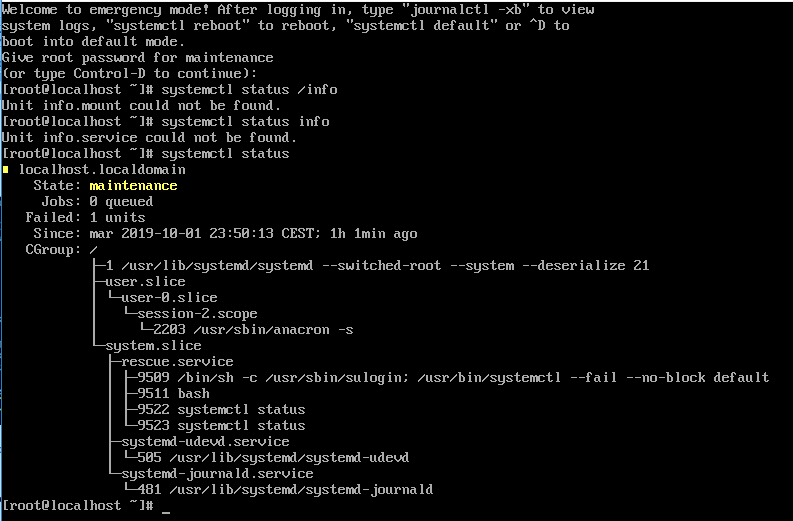
\includegraphics[width=0.8\linewidth]{images/i} 

}

\caption{Aspecto inicial del modo de mantenimiento (modo aislado).}\label{fig:i}
\end{figure}

\begin{enumerate}
\def\labelenumi{\arabic{enumi}.}
\setcounter{enumi}{10}
\tightlist
\item
  Ahora vamos a lo que queríamos hacer: copiar de \texttt{/var} a \texttt{/mnt/newvar}. Lo haremos (ver figura \ref{fig:j}) con \texttt{cp}, obviamente, y con la opción \texttt{–a} (para corregir errores de contexto de SELinux) y seleccionando \texttt{/var/.} (el detalle es el punto tras el \texttt{/var}, que indica que \emph{copie todo lo que haya, de manera recursiva y los ficheros ocultos incluidos}). Y lo comparamos con lo que hay en \texttt{/var} ejecutando: \texttt{\textgreater{}\ ls\ –lhaZ\ /var} y vemos que hay exactamente lo mismo, lo cual indica que hemos procedido correctamente.
\end{enumerate}

\begin{figure}

{\centering 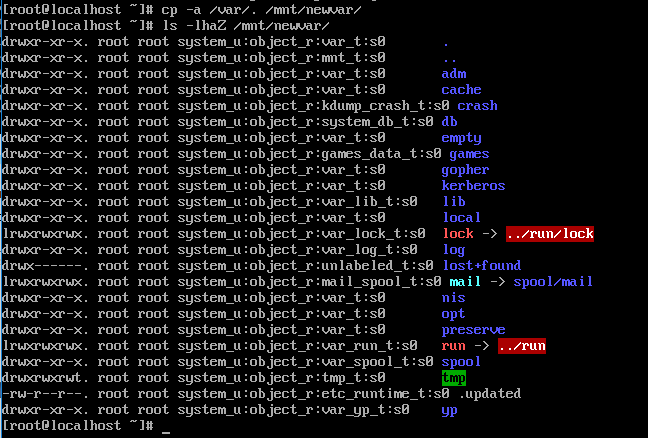
\includegraphics[width=0.75\linewidth]{images/j} 

}

\caption{Paso importante: copiando todo el contenido de `/var` a `/mnt/newvar` y comprobación con `ls`.}\label{fig:j}
\end{figure}

\begin{enumerate}
\def\labelenumi{\arabic{enumi}.}
\setcounter{enumi}{11}
\tightlist
\item
  Ahora falta decirle al sistema lo más importante: que cada vez que arranque, monte el volumen lógico \texttt{newvar} en \texttt{/var}, para que dicho cliente pueda seguir accediendo a \texttt{/var} de manera transparente a dónde estén sus archivos. Este es un paso delicado donde hay que modificar un archivo del sistema, el \texttt{/etc/fstab}, que da información sobre el montaje de dispositivos y particiones al arranque del Sistema Operativo. Lo haremos con extremo cuidado, usando el editor \texttt{vi} y en modo \textbf{root}.
\end{enumerate}

\begin{enumerate}
\def\labelenumi{\roman{enumi}.}
\tightlist
\item
  abrir el fichero \texttt{/etc/fstab} con \texttt{vi} usando la orden \texttt{sudo\ vi\ /etc/fstab}.
\item
  pulsamos la tecla \texttt{i} del teclado para acceder al modo de escritura,
\item
  vamos al final del fichero, insertamos una nueva línea (nos colocamos \textbf{al final} de la última línea y pulsamos \emph{Enter}),
\item
  insertamos en la nueva línea el siguiente contenido (donde la cadena \texttt{TABULADOR} indica que en ese lugar pulsemos la tecla de tabulador una sola vez):
\end{enumerate}

\begin{verbatim}
/dev/cl/newvarTABULADOR/varTABULADORext4TABULADORdefaultsTABULADOR0TABULADOR0
\end{verbatim}

\begin{enumerate}
\def\labelenumi{\alph{enumi}.}
\setcounter{enumi}{21}
\tightlist
\item
  tras repasar lo escrito y asegurarnos de que lo hemos escrito correctamente, pulsamos la tecla \texttt{Esc} para salir del modo de escritura y tecleamos en la línea de órdenes de la parte inferior de la pantalla que ofrece \texttt{vi} el literal \texttt{:wq} para guardar los cambios en el fichero (\texttt{w}) y salir (\texttt{q}).
\end{enumerate}

El aspecto final de \texttt{/etc/fstab} será el de la figura \ref{fig:k}.

\begin{figure}

{\centering 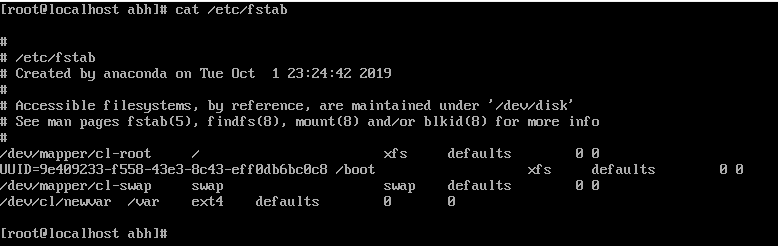
\includegraphics[width=0.95\linewidth]{images/k} 

}

\caption{Estado final de `/etc/fstab` tras las modificaciones oportunas.}\label{fig:k}
\end{figure}

\begin{enumerate}
\def\labelenumi{\arabic{enumi}.}
\setcounter{enumi}{12}
\item
  Desmontamos, para evitar posibles errores:

  \begin{enumerate}
  \def\labelenumii{\roman{enumii}.}
  \tightlist
  \item
    desmontar /mnt/newvar,
  \item
    y es posible que haga falta: desmontar /dev/cl/newvar
  \end{enumerate}
\item
  Ahora, mover \texttt{/var} a un directorio auxiliar llamado \texttt{/varold} (o el nombre que queramos) para evitar posibles errores. Ahora vamos a crear un nuevo \texttt{/var} mediante la orden \texttt{mkdir\ /var}, y le asignaremos un contexto a esa nueva carpeta con el comando de la figura \ref{fig:l}.
\item
  Ahora ya está todo hecho, sólo falta reiniciar la máquina y comprobar con \texttt{ls\ –lhaZ} que tanto \texttt{/var} como \texttt{/varold} tienen exactamente el mismo contenido.
\end{enumerate}

\begin{figure}

{\centering 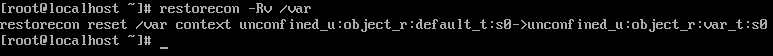
\includegraphics[width=0.95\linewidth]{images/l} 

}

\caption{Restaurar el contexto del nuevo directorio `/var`, donde montaremos nuestro nuevo disco `/dev/cl/newvar`.}\label{fig:l}
\end{figure}

\hypertarget{sesiuxf3n-3-ampliaciuxf3n-cifrada-y-redundante-de-la-capacidad-para-un-usuario.}{%
\section{Sesión 3: Ampliación cifrada y redundante de la capacidad para un usuario.}\label{sesiuxf3n-3-ampliaciuxf3n-cifrada-y-redundante-de-la-capacidad-para-un-usuario.}}

Este caso es una versión ``mejorada'' de la Sesión 2, pero hay que realizarla partiendo \emph{desde cero}, es decir, tras haber instalado centOS únicamente.

\begin{quote}
RECUERDA que esta sesión se realizará sobre una máquina virtual sobre la que NO se haya implementado lo realizado en la Sesión 2.
\end{quote}

\hypertarget{contextualizaciuxf3n-del-escenario-profesional-1}{%
\subsection{Contextualización del escenario profesional}\label{contextualizaciuxf3n-del-escenario-profesional-1}}

Tras ver el éxito de los vídeos alojados en el servidor configurado en la práctica anterior, un amigo de su cliente quiere proceder del mismo modo pero va a necesitar alojar información sensible así que le pide explícitamente que cifre la información y que ésta esté siempre disponible. Por tanto, la decisión que toma es configurar un RAID1 por software y cifrar el VL en el que /var estará alojado.

\hypertarget{quuxe9-necesitamos}{%
\subsection{¿Qué necesitamos?}\label{quuxe9-necesitamos}}

Aparte de lo mencionado antes sobre el Sistema Operativo y su estado, vamos a tener que crear dos discos extra, que serán los que conformen el RAID, uno de ellos tendrá el contenido exacto del otro (política de RAID1).

\hypertarget{pasos-para-la-realizaciuxf3n-de-la-pruxe1ctica}{%
\subsection{Pasos para la realización de la práctica}\label{pasos-para-la-realizaciuxf3n-de-la-pruxe1ctica}}

\begin{enumerate}
\def\labelenumi{\arabic{enumi}.}
\tightlist
\item
  Partimos inicialmente del estado original de centOS (puede estar la red configurada, no hay problema con eso) de la figura \ref{fig:1h}.
\end{enumerate}

\begin{figure}

{\centering 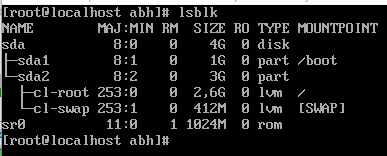
\includegraphics[width=0.75\linewidth]{images/1} 

}

\caption{Estado inicial antes de crear el RAID-1.}\label{fig:1h}
\end{figure}

\begin{enumerate}
\def\labelenumi{\arabic{enumi}.}
\setcounter{enumi}{1}
\tightlist
\item
  Entonces, vamos a apagar el sistema, añadimos los dos discos y reiniciamos. Lo que nos muestra ahora \texttt{lsblk} es lo siguiente (figura \ref{fig:2h}):
\end{enumerate}

\begin{figure}

{\centering 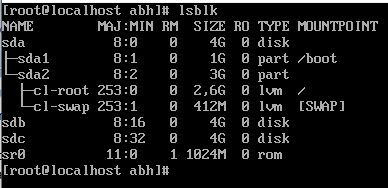
\includegraphics[width=0.75\linewidth]{images/2} 

}

\caption{Comando `lsblk` tras crear dos discos vírgenes.}\label{fig:2h}
\end{figure}

\begin{enumerate}
\def\labelenumi{\arabic{enumi}.}
\setcounter{enumi}{2}
\tightlist
\item
  Ahora vamos a crear directamente el dispositivo RAID-1 a partir de los dos discos sdb y sdc mediante un comando que se llama mdadm (multimedia-admin). Para instalarlo, ejecutamos \texttt{\textgreater{}\ yum\ install\ mdadm}. El resultado de este proceso se muestra en la figura \ref{fig:3h}, y vemos que nos muestra un error. Este fallo es por un error de conexión a la red. Lo comprobamos ejecutando \texttt{ipaddr}, y vemos que la interfaz \texttt{enp0s3} (la que tenemos que mirar en nuestro caso para conectarnos a Internet) no tiene IP asignada. Hay que levantar la red mediante el comando \texttt{ifup\ enp0s3}; en la figura \ref{fig:4h} vemos que ya se \emph{levantado} correctamente.
\end{enumerate}

\begin{figure}

{\centering 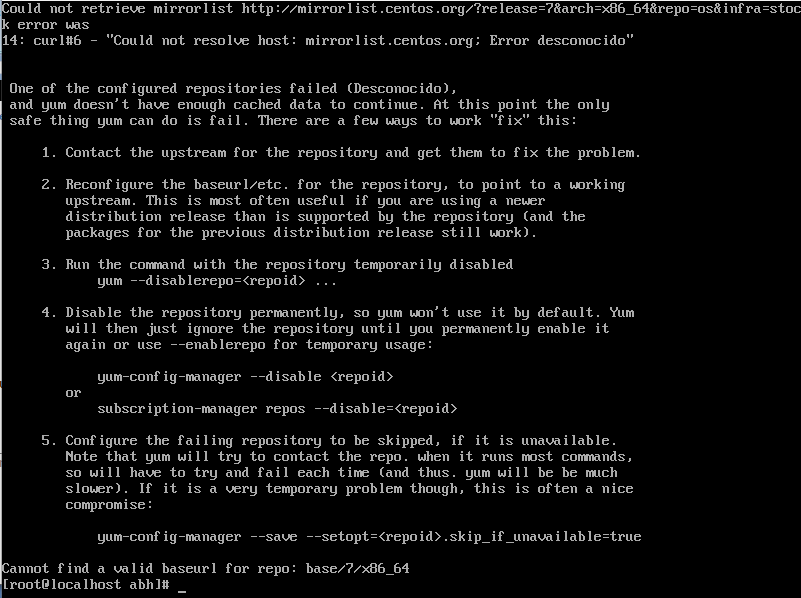
\includegraphics[width=0.9\linewidth]{images/3} 

}

\caption{Comando `lsblk` tras crear dos discos vírgenes.}\label{fig:3h}
\end{figure}

\begin{figure}

{\centering 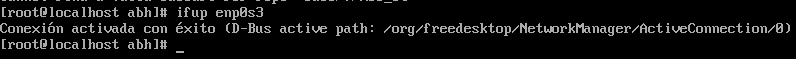
\includegraphics[width=0.95\linewidth]{images/4} 

}

\caption{Comando `lsblk` tras crear dos discos vírgenes.}\label{fig:4h}
\end{figure}

\begin{enumerate}
\def\labelenumi{\arabic{enumi}.}
\setcounter{enumi}{3}
\item
  Tras conectarnos setisfactoriamente a Internet, ahora ya podremos instalar el gestor de RAID con el comando \texttt{\textgreater{}\ yum\ install\ mdadm}, decimos que sí a todo (opción \texttt{y}) y se instalará.
\item
  \textbf{Creación del RAID-1}. Para crearlo correctamente y con las opciones que queramos habría que mirar el manual en línea de \texttt{mdadm}. Tras el correspondiente estudio, las opciones que más nos convienen se muestran en la orden de la figura \ref{fig:5h}.
\end{enumerate}

\begin{figure}

{\centering 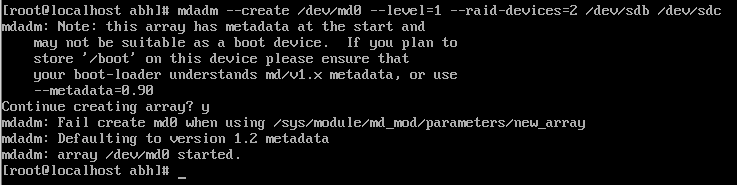
\includegraphics[width=0.95\linewidth]{images/5} 

}

\caption{Creando el RAID-1 a partir de los discos `sdb` y `sdc`.}\label{fig:5h}
\end{figure}

\begin{enumerate}
\def\labelenumi{\arabic{enumi}.}
\setcounter{enumi}{5}
\tightlist
\item
  El comando \texttt{lsblk} nos muestra si hemos creado correctamente el RAID-1 (ver figura \ref{fig:6h}.
\end{enumerate}

\begin{figure}

{\centering 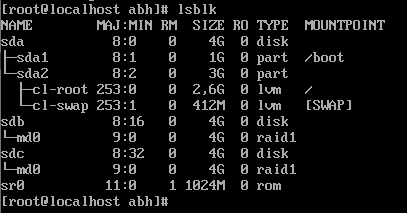
\includegraphics[width=0.75\linewidth]{images/6} 

}

\caption{Resultado del comando `lsblk` tras crear el RAID-1.}\label{fig:6h}
\end{figure}

\begin{enumerate}
\def\labelenumi{\arabic{enumi}.}
\setcounter{enumi}{6}
\tightlist
\item
  Ahora creamos el volumen físico que podemos llamar \texttt{newvar} y que servirá de base para el grupo de volúmenes del RAID con la orden \texttt{pvcreate\ /dev/md0} y comprobamos que se ha creado correctamente como ya sabemos.
\item
  Creamos el grupo de volúmenes con \texttt{vgcreate\ pmraid1\ /dev/md0}. Después creamos el volumen \textbf{lógico} (que se duplicará mediante la técnica RAID) de 1 GB de tamaño con: \texttt{lvcreate\ –L\ 1G\ –n\ newvar\ pmraid1}. Veamos cómo va todo con \texttt{pvs}, \texttt{vgs} y \texttt{lvs}, cuyas salidas se muestran en la figura \ref{fig:7h}.
\end{enumerate}

\begin{figure}

{\centering 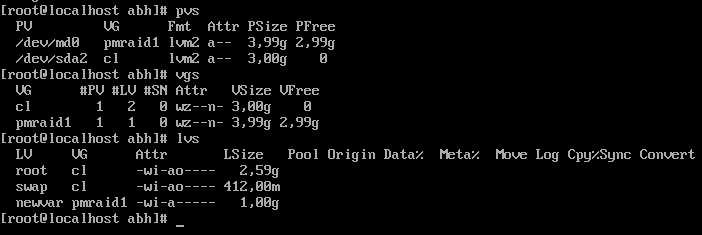
\includegraphics[width=0.95\linewidth]{images/7} 

}

\caption{Estado tras crear el volumen lógico `newvar`.}\label{fig:7h}
\end{figure}

\begin{enumerate}
\def\labelenumi{\arabic{enumi}.}
\setcounter{enumi}{8}
\tightlist
\item
  En este punto, recordemos cuál era nuestro objetivo: crear una nueva unidad lógica \textbf{redundante} y \textbf{encriptada}. Solo nos falta la encriptación. Esto lo haremos con el comando \texttt{cryptsetup} y algunas opciones del mismo. Lo primero, vamos a instalarlo con \texttt{yum\ install\ cryptsetup} (esto no debe dar errores). Ahora entraremos en modo aislado con \texttt{\%\ systemctl\ isolate\ runlevel1.target}, y ahí ejecutamos los siguientes comandos, en el orden dado (figura \ref{fig:8h}).
\end{enumerate}

\begin{figure}

{\centering 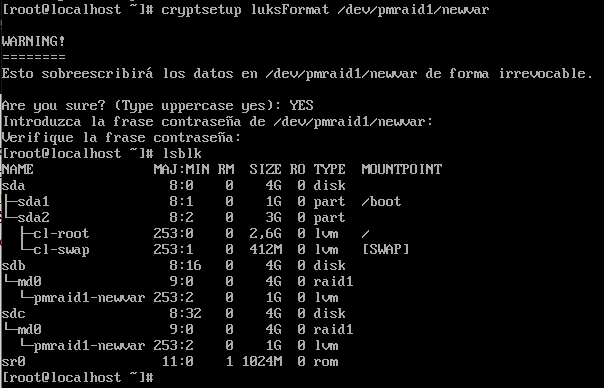
\includegraphics[width=0.75\linewidth]{images/8} 

}

\caption{Resultado de la encriptación.}\label{fig:8h}
\end{figure}

\begin{enumerate}
\def\labelenumi{\arabic{enumi}.}
\setcounter{enumi}{9}
\tightlist
\item
  ¿Qué ha pasado? Que hemos encriptado satisfactoriamente el volumen \texttt{newvar}, pero la zona encriptada dentro de ese volumen no está abierta (\emph{accesible}), y entonces \texttt{lsblk} no lo reconoce. Abrámoslo con el comando siguiente, asignémosle un nombre que nos ayude a identificarlo (\texttt{pmraid1-newvar\_crypt}), y después \texttt{lsblk} ya lo conocerá. Lo vemos en la figura \ref{fig:9h}.
\end{enumerate}

\begin{figure}

{\centering 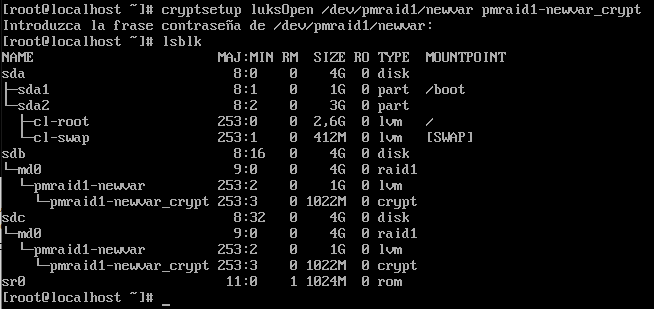
\includegraphics[width=0.95\linewidth]{images/9} 

}

\caption{Resultado de abrir la zona encriptada del volumen. Mostramos el resultado con `lsblk`, donde ya aparece ese volumen encriptado con el nombre que le hemos puesto en el comando.}\label{fig:9h}
\end{figure}

\begin{enumerate}
\def\labelenumi{\arabic{enumi}.}
\setcounter{enumi}{10}
\item
  Ahora quedan tareas que ya conocemos (salvo una que veremos después):

  \begin{enumerate}
  \def\labelenumii{\alph{enumii}.}
  \tightlist
  \item
    vamos a asignar un sistema de archivos a ese volumen encriptado (que no al \texttt{newvar}) con el comando
  \end{enumerate}

\begin{verbatim}
mkfs –t ext4 /dev/mapper/pmraid1-newvar_crypt
\end{verbatim}

  \begin{enumerate}
  \def\labelenumii{\alph{enumii}.}
  \setcounter{enumii}{1}
  \tightlist
  \item
    ahora lo montamos en un directorio auxiliar de \texttt{/mnt}, por ejemplo \texttt{/mnt/varcifr}, y le copiamos todos los archivos. Veamos estas operaciones ejecutadas (ver figura \ref{fig:10h}):
  \end{enumerate}
\end{enumerate}

\begin{figure}

{\centering 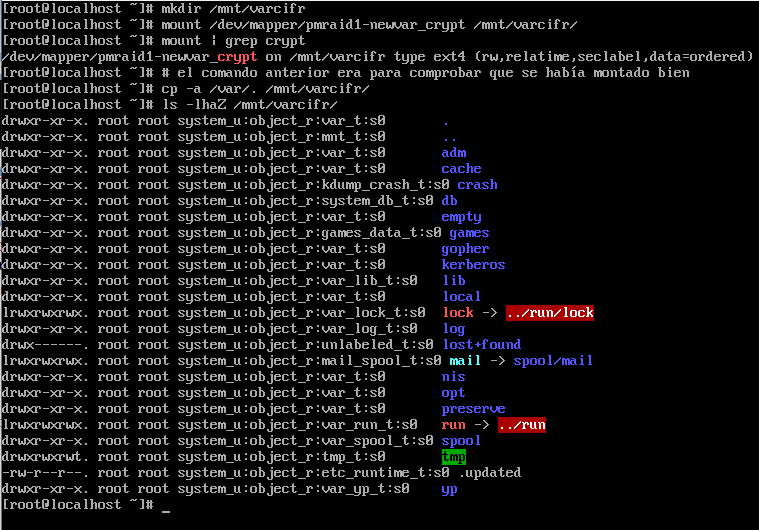
\includegraphics[width=0.95\linewidth]{images/10} 

}

\caption{Operaciones de montaje del dispositivo cifrado para copiarle los archivos en un punto de montaje temporal. Todos los pasos se van comprobando.}\label{fig:10h}
\end{figure}

\begin{enumerate}
\def\labelenumi{\arabic{enumi}.}
\setcounter{enumi}{11}
\item
  Usamos un fichero llamado \texttt{/etc/crypttab}, el cual especifica en el arranque como se deben descifrar los discos. Para ello usaremos el nombre (sin el \emph{path}) del volumen encriptado (es decir, \texttt{pmraid1-newvar\_crypt}), el \emph{identificador único universal} (UUID), el \emph{tipo} del sistema de archivos y la \emph{etiqueta} (si está configurada). En ese fichero añadiremos esta información para especificar al sistema como descifrar este disco.

  \begin{enumerate}
  \def\labelenumii{\alph{enumii}.}
  \tightlist
  \item
    Coger del comando \texttt{crypto} la información del volumen y volcarla en una nueva línea del fichero \texttt{/etc/crypttab}:
  \end{enumerate}

\begin{verbatim}
grep crypto >> /etc/crypttab
\end{verbatim}

  \begin{enumerate}
  \def\labelenumii{\alph{enumii}.}
  \setcounter{enumii}{1}
  \tightlist
  \item
    Ahora podemos usar \texttt{vi} para abrir este fichero y modificar la línea que acabamos de añadir para colocar, \textbf{al principio} de la misma, la cadena \texttt{pmraid1-newvar\_crypt} (nótese el espacio al final, para separarlo del resto del contenido de la línea).
  \end{enumerate}
\item
  Ahora modificamos el fichero \texttt{/etc/fstab} para que quede como en la figura \ref{fig:13h}.
\end{enumerate}

\begin{figure}

{\centering 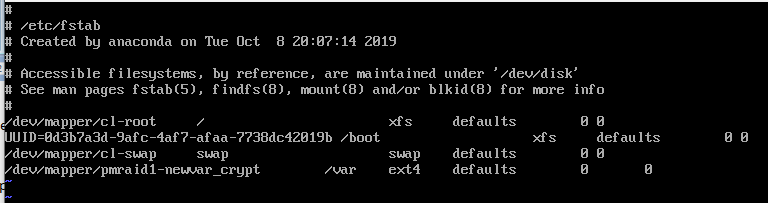
\includegraphics[width=0.8\linewidth]{images/13} 

}

\caption{Estado final del fichero `/etc/fstab`.}\label{fig:13h}
\end{figure}

\begin{enumerate}
\def\labelenumi{\arabic{enumi}.}
\setcounter{enumi}{13}
\tightlist
\item
  Ahora nos queda una tarea importante, que es preparar el directorio \texttt{/var} para que el usuario pueda acceder a él, para lo cual tenemos que:

  \begin{enumerate}
  \def\labelenumii{\alph{enumii}.}
  \tightlist
  \item
    crear un directorio auxiliar donde almacenar el contenido de \texttt{/var}:
  \item
    liberar el espacio de \texttt{/var}:
  \item
    \emph{``todo lo que se monta, se desmonta''}: desmontamos el volumen \texttt{/mnt/varcifr}:
  \item
    crear el nuevo directorio para el usuario, \texttt{/var}:
  \item
    y restauramos el contexto de este nuevo directorio:
  \end{enumerate}
\item
  Ahora podemos reiniciar el servidor, ejecutar
\end{enumerate}

\begin{verbatim}
mount | grep crypt
\end{verbatim}

y ver que se ha montado satisfactoriamente el volumen encriptado.

\hypertarget{instalaciuxf3n-y-configuraciuxf3n-de-servicios}{%
\chapter{Instalación y configuración de servicios}\label{instalaciuxf3n-y-configuraciuxf3n-de-servicios}}

\hypertarget{monitorizaciuxf3n-y-automatizaciuxf3n-de-tareas}{%
\chapter{Monitorización y automatización de tareas}\label{monitorizaciuxf3n-y-automatizaciuxf3n-de-tareas}}

\hypertarget{objetivos}{%
\section{Objetivos}\label{objetivos}}

\begin{enumerate}
\def\labelenumi{\arabic{enumi}.}
\tightlist
\item
  Conocer y saber usar las herramientas que permitan obtener datos sobre el sistema a nivel hardware y software (SO y servicios).
\item
  Saber interpretar los resultados proporcionados por las aplicaciones de monitorización.
\item
  Conocer los archivos que proporcionan información del sistema.
\item
  Tener conocimiento básico sobre automatización y orquestación
\item
  Ser capaz de utilizar y configurar un monitor de sistema
\end{enumerate}

\hypertarget{introducciuxf3n}{%
\section{Introducción}\label{introducciuxf3n}}

El guión de prácticas asociado a este documento contiene una información interesante, que además es materia \textless{}\textgreater{} sobre los monitores disponibles, su clasificación, además de algunos temas muy interesantes sobre Automatización y Profiling del sistema.

En el presente documento nos centraremos en resolver las tareas evaluables propuestas para esta práctica: monitorización con Zabbix y automatización básica de tareas con Ansible.

\hypertarget{sesiuxf3n-1uxaa-automatizaciuxf3n-buxe1sica-de-tareas-con-ansible}{%
\section{Sesión 1ª: Automatización básica de tareas con Ansible}\label{sesiuxf3n-1uxaa-automatizaciuxf3n-buxe1sica-de-tareas-con-ansible}}

\hypertarget{introducciuxf3n-a-la-orquestaciuxf3n-con-ansible}{%
\subsection{Introducción a la orquestación con Ansible}\label{introducciuxf3n-a-la-orquestaciuxf3n-con-ansible}}

En el guión oficial de esta práctica se indicaban varias herramientas para la automatización de tareas. Una de ellas, que actúa a nivel de plataforma es Ansible.

Ansible es un software que automatiza el \textbf{aprovisionamiento} de \emph{software}, la gestión de configuraciones y el despliegue de aplicaciones. Está categorizado como una herramienta de \emph{orquestación}, muy útil para los administradores de sistema y DevOps\footnote{DevOps es una metodología de desarrollo de \emph{software} basada en la integración entre desarrolladores \emph{software} y administradores de sistemas}.

En otras palabras, Ansible permite a los DevOps gestionar sus servidores, configuraciones y aplicaciones de forma sencilla, robusta y paralela

Tal y como se indica en , ``{[}Ansible{]} gestiona nodos a través de SSH y no requiere ningún software remoto adicional (excepto Python 2.4 o posterior para instalarlo)''.

En definitiva, hablamos de una herramienta para:
- automatizar tareas,
- provisional, y
- orquestar servicios (a esto nos dedicaremos a continuación).

\hypertarget{pruebas-sobre-nuestras-muxe1quinas-virtuales}{%
\subsection{Pruebas sobre nuestras máquinas virtuales}\label{pruebas-sobre-nuestras-muxe1quinas-virtuales}}

Para realizar las pruebas podemos usar las dos máquinas virtuales que tenemos: Ubuntu y centOS. Basta con ejecutar los comandos en una máquina apropiadamente para que se ejecute en la otra, logrando la comunicación entre ambos.

Para la prueba no hace falta realmente iniciar sesión en la máquina virtual que recibirá las órdenes de ejecución; sólo habrá que hacerlo donde vayamos a lanzar los comandos.

\begin{enumerate}
\def\labelenumi{\arabic{enumi}.}
\item
  Instalar Ansible en Ubuntu: ejecutaremos el comando:

\begin{verbatim}
sudo apt install ansible
\end{verbatim}
\item
  Creación de grupos \emph{receptores} de tareas: En el fichero \texttt{/etc/ansible/hosts} se pueden definir los \emph{receptores} y grupos de los mismos de las tareas que vayamos a lanzar con Ansible.

  Para definir un grupo de destinos basta con indicar un nombre de referencia entre corchetes, y debajo, en cada línea, el formato \texttt{IP:PUERTO} del host destino. Un formato válido para un grupo básico sería:

\begin{verbatim}
[UbuntuServer]
192.168.56.105:22022
[centOSServer]
192.168.56.110:22022
\end{verbatim}

  en el caso de que quisiéramos un grupo para cada servidor (un grupo para el servidor \emph{Ubuntu} y otro grupo para el de \emph{centOS}).
\item
  Lanzar tareas desde Linux (anfitrión o máquina virtual): Mandar la orden de hacer ping\} a todos los grupos de servidores que hayamos definido en el fichero /etc/ansible/hosts\}:
\end{enumerate}

\begin{verbatim}
ansible all -m ping  # all = mandar a todos los grupos
\end{verbatim}

Es posible que nos dé un error, debido a problemas con la clave público-privada. Podemos solucionar este problema generando una clave con la orden

\begin{verbatim}
ssh-keygen
\end{verbatim}

y se generan las claves (pública y privada)\footnote{Refresca los conocimientos sobre criptografía necesarios para las prácticas en el documento asociado a la Práctica 2 (elaboración propia).\} en el fichero .ssh/} (carpeta oculta en el directorio actual).

Ahora nos falta enviar la clave a los destinatarios uno a uno con

\begin{verbatim}
ssh-copy-id IP -p PUERTO
\end{verbatim}

Si volvemos a ejecutar el comando de \emph{Ansible}, puede que nos vuelva a dar un error relacionado con Python. Lo podemos solucionar instalándolo con:

sudo apt install python \# suponiendo que estamos en Ubuntu
apt update \# actualizar repositorios
\textbackslash end\{lstlisting\}

Ahora volvemos a ejecutar el comando (ver figura ).

\hypertarget{benchmarking-y-ajuste-del-sistema-profiling}{%
\chapter{\texorpdfstring{\emph{Benchmarking} y ajuste del sistema (\emph{profiling})}{Benchmarking y ajuste del sistema (profiling)}}\label{benchmarking-y-ajuste-del-sistema-profiling}}

Some \emph{significant} applications are demonstrated in this chapter.

\hypertarget{example-one}{%
\section{Example one}\label{example-one}}

\hypertarget{example-two}{%
\section{Example two}\label{example-two}}

\hypertarget{final-words}{%
\chapter{Final Words}\label{final-words}}

We have finished a nice book.

  \bibliography{book.bib,packages.bib}

\end{document}
